% !TeX root = ../../../../../../thesis.tex



\subparagraph{Current Source}



	To solve the issue of the non-constant current draw of the other LED solutions, a current source will be used to power the LED.
	The principle is the same as in the DC environment, where also a current source is used.
	In \autoref{fig:custom-modulator-current-source} the schematic for the current source implementation can be seen.
	An optocoupler is used to electrically isolate and protect the micro-controller from the current source, during the development stages.


	\begin{figure}[ht]
		\centering
		\begin{minipage}[b]{0.49\textwidth}
			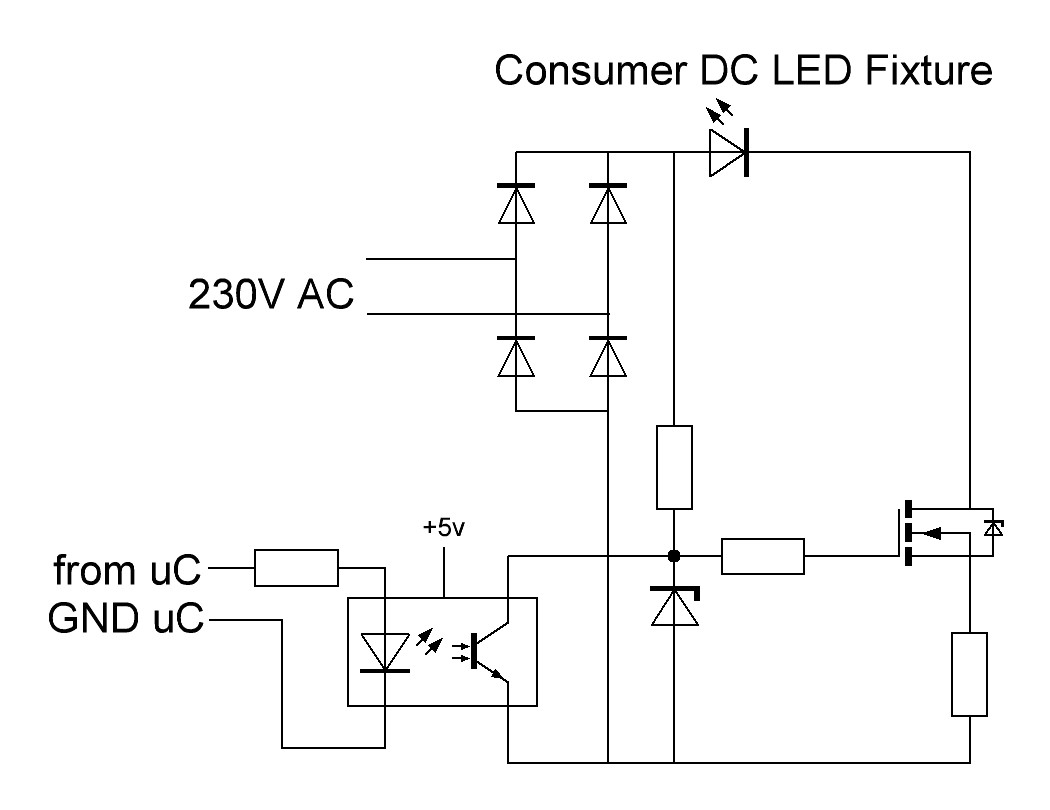
\includegraphics[width=\textwidth]{chapters/hardware-chapters/AC/ac-modulator/custom-hardware/ac-current-source/custom-modulator-current-source.JPG}
			\caption{Current source to power the commercial LED fixture, can be toggled on and off with a microprocessor.}
			\label{fig:custom-modulator-current-source}
		\end{minipage}
		\hfill
		\begin{minipage}[b]{0.49\textwidth}
			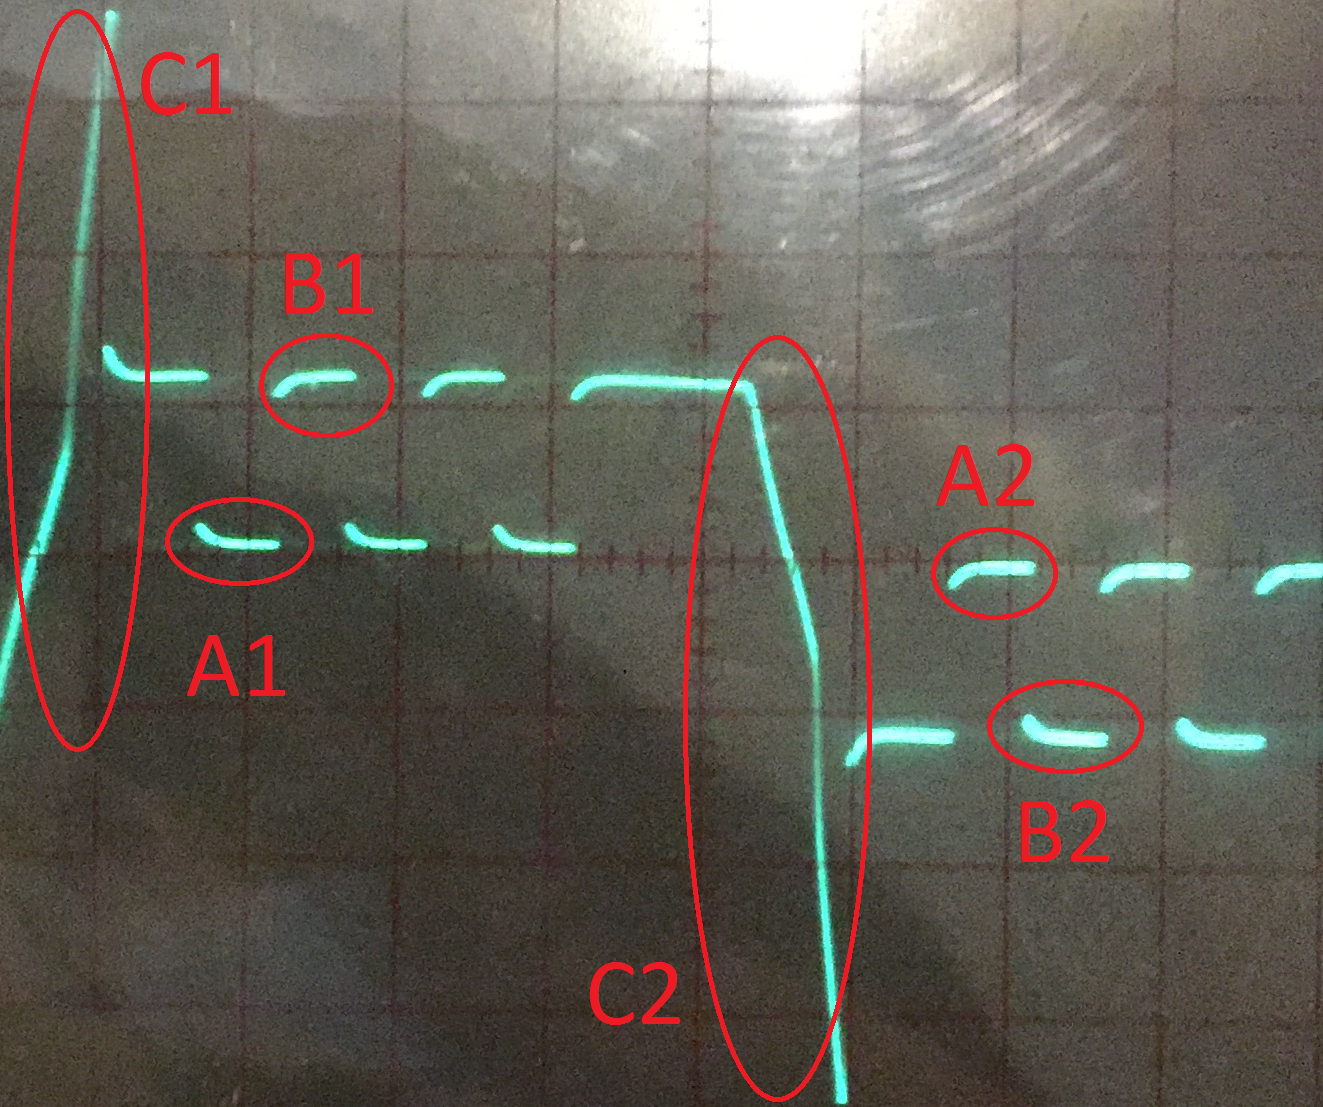
\includegraphics[width=\textwidth]{chapters/hardware-chapters/AC/ac-modulator/custom-hardware/ac-current-source/current-source-measurement-annotated.png}
			\caption{Current that is drawn by the current source. Measured over an 2.8 Ohm resistor. Settings: 200 mV/div, 2 ms/div.}
			\label{fig:current-source-measurement-annotated}
		\end{minipage}
	\end{figure}




	To investigate exactly how the current source implementation performs, a 2.8 Ohm resistor is placed in series with the AC and the current source implementation.
	A micro-controller will toggle the current source on and off via the optocoupler with a frequency of 500 Hz.
	This relatively low frequency is chosen to show the distinct on and off states of the current.
	If a higher frequency was chosen, the on and off state are harder to see on the figure.
	The voltage drop over the series resistor is measured to determine the current draw.
	The result of the current draw can be seen in \autoref{fig:current-source-measurement-annotated}.

	


	In \autoref{fig:current-source-measurement-annotated} six areas are highlighted.
	The regions highlighted with a `1' suffix occur when the supplied AC voltage is positive and the regions with a `2' suffix occur when the AC voltage is negative.
	What happens in these regions will now be explained:


	\begin{itemize}

		\item In region A1 and A2, the LED is turned off because the micro-controller is encoding a `0' and we can see that the current draw is also zero.
		The current draw is zero, independent if the applied AC voltage is positive, in A1, or negative, in A2.


		\item In region B1 and B2, the LED is on, the micro-controller is encoding a `1'. 
		In both regions the current draw remains constant over time, until the LED is turned off.
		But in B1, the current is a positive constant and in B2 the current is a negative constant.
		This is due to the applied AC voltage.
		%In B1 the voltage is positive, so a positive current will flow.
		%And in B2, the voltage is negative, so a negative current will flow.

		\item What happens in regions C1 and C2 is caused by a voltage source, which powers parts of the triggering circuit and the current source.
		What exactly is happening will be explained in the next section, but for now we can assume that it will not affect the encoding of the ID.

	\end{itemize}




	The combination of the trigger circuit and this implementation of a current source allows this solution to detect when to start and stop modulating the LED and it is able to define a specific current draw for the LED.
	This makes mapping the bits `0' and `1' to current levels zero and some constant, easy.
	Which in turn makes detecting the IDs of the LEDs in the smart-meter easy. %which receives an aggregated current, possible.

	






	However, this solution also has a drawback.
	The current source will make sure a constant amount of current will flow through the LEDs.
	The current that flows through the LEDs will cause a voltage difference over the LEDs.
	This is the voltage the LEDs need in order for current to flow, as discussed in the previous sections.
	In the triggering circuit section, it was explained that the LEDs used, require 100 V before the current will flow, see \autoref{fig:triggering-circuit-output-2}.
	This voltage is all the voltage that is needed for these LEDs.
	If less voltage is provided, the LEDs will not emit light.
	But more voltage than necessary will result in power dissipation in some component and will turn into heat.
	Since the applied AC voltage is rated at 230 V RMS, the excessive voltage has to go somewhere.
	This voltage will be dissipated over the current source.
	This means that some energy is being wasted, because there is more voltage provided by the AC than is needed to power the LEDs.



	The other LED solutions discussed above (SMPS LED and 230 V AC LED), solve this problem is two separate manners.
	The SMPS LED, uses a power supply to transform the supplied AC voltage to a certain DC voltage which is exactly what the LEDs need.
	The SMPS has a high efficiency so no power is being wasted, but at the same time this power supply disturbs the encoding of the ID in such a way that the ID is not recognizable anymore.
	The 230 V AC LED uses many LEDs in series and so it requires a very high voltage before the LEDs turn on.
	So only a limited amount of time is used to turn the LEDs on and therefore only a small amount of time is available for modulation of the ID.
	And in the process of encoding the ID, the current is not constant and it does not produce a square wave which makes recognizing the ID difficult.


	The current source implementation, as discussed in this section, solves the encoding problems which the other solutions had.
	But this solution introduces an efficiency problem.
	The priority of this thesis was to create a solution which could recognize which LEDs are on and off by only looking at the aggregated energy consumption.
	The efficiency of this solution has a lower priority. %, which is why this solution was still chosen to develop.
	However, attempts have been made to try and solve the efficiency problem.
	The first attempt involves the use of a transformer and the second attempt uses a capacitor.

	\begin{figure}[htb]
		\centering
		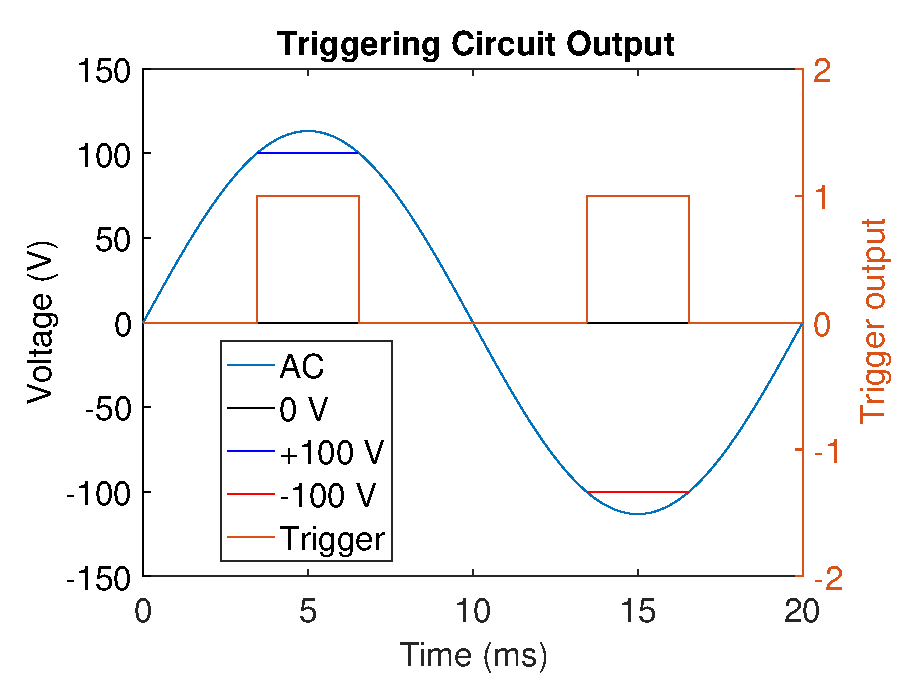
\includegraphics[angle=0,width=0.5\textwidth]{chapters/hardware-chapters/AC/ac-modulator/custom-hardware/ac-current-source/ac-wave-lower-transformed-triggering.eps}
		\caption{Output triggering circuit alongside the output of the AC voltage after a transformer.}
		\label{fig:trigger-output-lower-transformed}
	\end{figure}


	The first attempt uses a transformer to transform the 230 V AC to a lower AC voltage which will solve the efficiency problem.
	The outputted sine wave of the transformer can be seen in \autoref{fig:trigger-output-lower-transformed}.
	The LEDs still need the same amount of voltage: 100V.
	This 100 V threshold can also be seen in \autoref{fig:trigger-output-lower-transformed}.
	The time that is now available for modulation is limited by the use of the transformer, and is 6 ms, which means that only $\frac{6}{20} = 30$ \% of the time is available for modulation.
	Another drawback of using a transformer, is that the distinct current signature that is made using the ID, is distorted by the transformer, as no ideal transformer exists.
	For this reason this solution was abandoned.





	The second attempt showed promising results, however due to time constraints it was not possible to fully investigate this solution. 
	The solution is made up out of two parts: A capacitor and a zero-crossing optotriac.
	The capacitor is placed in series with incoming AC to the rectifying bridge.
	And the optotriac is parallel to this capacitor.
	The schematic can be seen in \autoref{fig:ac-capacitor-triac}.

	\begin{figure}[ht]
		\centering
		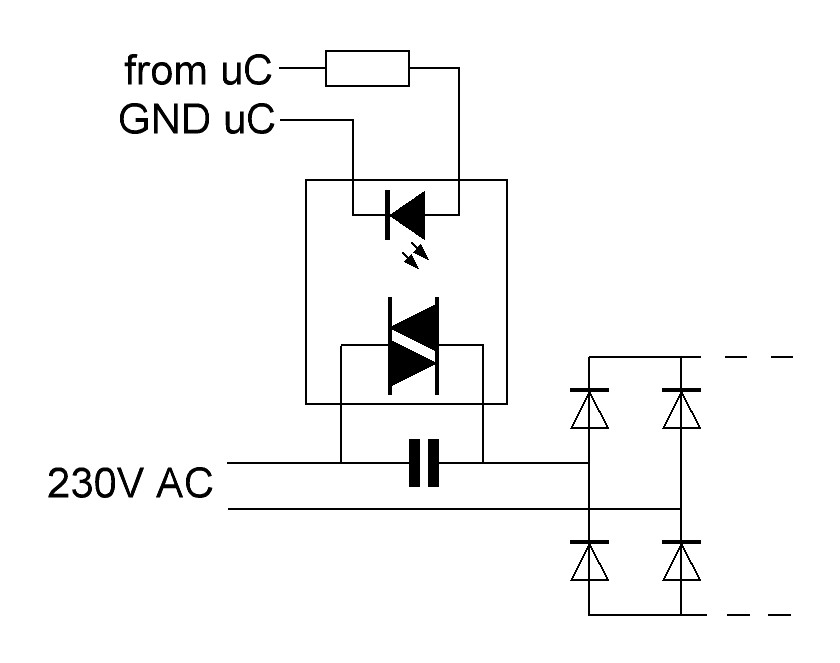
\includegraphics[angle=0,width=0.4\textwidth]{chapters/hardware-chapters/AC/ac-modulator/custom-hardware/ac-current-source/ac-capacitor-triac.JPG}
		\caption{Schematic to show how the capacitor and optotriac are connected.}
		\label{fig:ac-capacitor-triac}
	\end{figure}

	The series capacitor will limit the power that can be dissipated by the current source.
	The capacitor is able to do this by phase shifting the current as seen from the voltage.
	%In this process the current itself will not be distorted as was the case with using a transformer as discussed above and so the distinct current signature will still be intact.
	The voltage drop over the capacitor can be calculated using Ohm's law $U = R \times I$ and the resistance of a capacitor which is called the reactance, $X_c$ measured in ohms.
	The reactance of a capacitor is dependent on the frequency of the voltage $f$ and the capacitance $C$: $X_c = \frac{1}{\omega \times C} = \frac{1}{2 \times \pi \times f \times C}$.
	The frequency of the voltage is 50 Hz, because the AC power is rated at 50 Hz.
	Since a current source is used to power the LED, the current will be a constant value when the LED is on.
	The voltage drop can be calculated by assuming a current of $0.1$ A and a standard capacitance value of 3.3 $\mu$F.
	The voltage drop will then be: $U = R \times I = X_c \times I = \frac{1}{2 \times \pi \times f \times C} \times I = \frac{1}{2 \times \pi \times 50 \times 3.3 \times 10^{-6}} \times 0.1 = 96.5$ V.
	This means that the voltage applied to the modulator circuit will now be lowered by approximately 100 V.
	Even though there is a voltage drop over the capacitor, the capacitor itself will not dissipate any power.
	This is because the capacitor has no resistance, the real part of the impedance is zero, but it only has reactance which is the imaginary part of the impedance.
	Due to the voltage drop the efficiency problem can be solved.
	However by limiting the voltage that the current source can use, there is much less time available to modulate, similar to the solution with the transformer as described above, see \autoref{fig:trigger-output-lower-transformed}.
	This is were the zero-crossing triac comes in.
	If the probabilistic approach is used, the LED is not constantly transmitting its code, instead most of the time it is not modulating.
	Whenever it is decided to start modulating by the probabilistic approach, the micro-controller activates the triac and then it will short-circuit the capacitor.
	When this happens, effectively the capacitor is no longer connected and it no longer limits the voltage.
	And so the time available for modulation is restored to the full 80 \%.
	When the transmission of the ID of the LED is finished, the triac is switched off and the capacitor limits the power once again.
	During the transmission of the ID, the current source is dissipating power, but this is only during the transmission of the ID, which is the amount of time to encode the ID.
	Whenever the LED is not transmitting its ID, the capacitor is limiting the voltage and thus the efficiency issue is solved.
	But due to time constraints it was not possible to fully investigate this solution with the testbed.	


